\chapter{Methodik}
\label{chap:methodik} Wie das vorherige Kapitel bereits eingeleitet hat, soll es
hier um das \textit{Wie} gehen. Es wird also aufgezeigt, welches methodische Herangehen
an die Fragestellung verfolgt wurden, um ein aussagekräftiges Ergebnis zu
erzielen. Dabei wurde mit einer umfangreichen Anforderungsanalyse gestartet,
welche die Domäne und die Ausgangslage klären soll. Sind diese Konzepte klar, so
wird die endgültige Problemstellung in mehrere kleine Teilaufgaben zerlegt. Für jede
dieser Teilaufgaben wurde dann eine Recherche zum Stand der Technik durchgeführt,
um bereits existierenden Lösungen ausfindig zu machen. Sofern es für eine Teilaufgabe
noch keine Lösung gibt, werden anschließend konkrete Lösungsansätzen für die
einzelnen Teilprobleme erarbeitet. Sollte für eine Aufgabe mehrere Ansätze existieren,
so werden diese im letzten Abschnitt miteinander verglichen und ein passender
Ansatz gewählt.

Bei der Durchführung dieser Schritte zum Erreichen eines Ergebnisses, soll der in
der Softwareentwicklung allgemeine bekannte Ansatz \textit{make it run, make it right,
make it fast} verfolgt werden. Dieser beschreibt, dass zunächst dafür gesorgt
werden soll, dass ein Problem überhaupt gelöst wird, bevor man viel Zeit in ein
Refactoing oder eine Optimierung steckt.
% ---------------------------------------------------------------------------------------

\section{Anforderungsanalyse}
\label{sec:anforderungsanalyse} Nach genauerem Betrachten der Fragestellung aus
Kapitel \ref{chap:fragestellung} wird klar, dass im Rahmen dieser vorliegenden Arbeit
eine Extension für die Plattform 3D Slicer entwickelt werden soll. Diese
Erweiterung beinhaltet das Segmentierungsverfahren nach Hoffmann \citep[vgl.][]{hoffmann2020},
wie es in Kapitel \ref{sec:verwwandte_arbeit} beschrieben wurde. Das Verfahren segmentiert
Micro-CT Aufnahmen der Zahnklinik in München und wird zu Forschungszwecke eingesetzt.
Da Ärzte keine Softwareentwickler sind, ist es wichtig, dass das Verfahren eine
UI erhält die eingängig und übersichtlich ist. Außerdem ist eine stabile Anwendung
gefragt, die sich gut in die Kernanwendung von 3D Slicer einfügt. Für einen Überblick
über die wichtigsten Eigenschaften von 3D Slicer sei auf das Kapitel \ref{sec:3d_slicer}
verwiesen.

Die Extension selber soll neben einer Einzelbildbearbeitung auch einen Batch-Prozess
ermöglichen. So können Beispielsweise Parameter an einem Bild erprobt werden und
diese anschließend in eine Batchprozess für viele Bilder überführt werden. Außerdem
soll es möglich sein, verschiedenen Segmentierungsverfahren, die in Hoffmann vorgesehen
sind, auch in der Extention auszuwählen.

Ein wichtiger Softwaretechnischer Anspruch an die Extension ist die
Erweiterbarkeit. Es soll ohne große Mühen möglich sein, ein weiteres Verfahren
zu integrieren, ohne das große Anpassungen an der UI oder der Erweiterung selbst,
unternommen werden müssen. Für ein solides Verständnis dieser Software soll es selbstverständlich
eine Dokumentation mit Benutzerhandbuch geben. Zudem wird großer Wert auf die
Qualitätssicherung gelegt, weshalb eine Reihe von Unit-Tests (Tests für einzelne
Programmeinheiten) vorgesehen ist.

Um die Anforderungen an die Software besser zu verstehen und zu strukturieren,
ist neben der Sammlung technischer Spezifikationen auch ein solides Verständnis
für die zugrunde liegende Domäne essenziell. Die Abbildung \ref{fig:3d_slicer_domäne}
veranschaulicht dies durch ein UML-Domänenmodell (Unified Modeling Language),
das einen visuellen Überblick über die verschiedenen Teile der Software bietet. Dazu
sind auch einige Anforderungen wieder zu erkennen.

\begin{figure}[h]
	\centering
	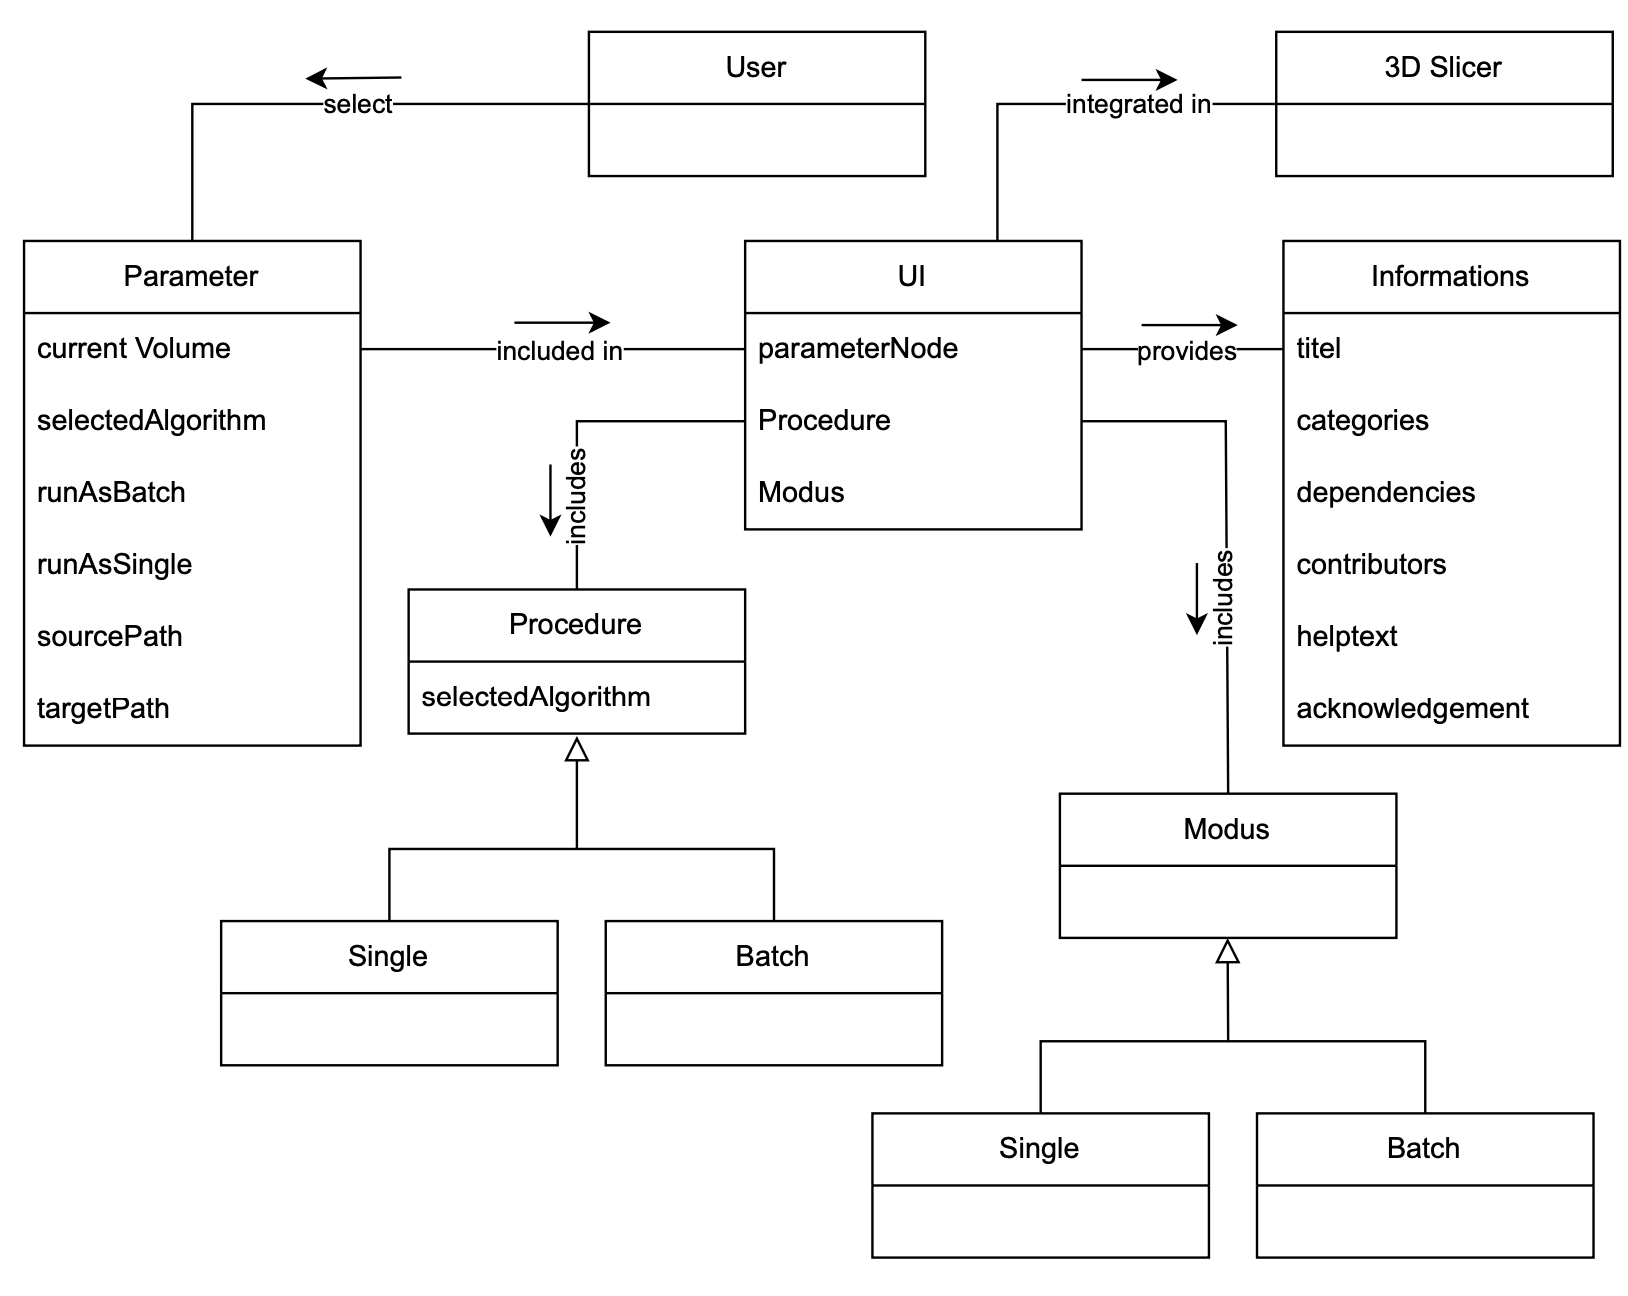
\includegraphics[width=0.8\textwidth]{img/domaenenmodell.jpg}
	\caption{UML-Domänenmodell des gesamten Softwaresystems}
	\label{fig:3d_slicer_domäne}
\end{figure}

Diese doch breite Palette an Anforderungen lässt sich unmöglich auf einmal
bearbeiten. Auch durch eine visuelle Darstellung kann dies nicht vereinfacht werden.
Hierzu sieht diese Arbeit eine Aufteilung in Teilprobleme vor. Der nächste Abschnitt
blickt auf die herausgearbeiteten Anforderungen in diesem Kapitel und leitet daraus
Teilprobleme ab.
% ---------------------------------------------------------------------------------------

\section{Zerlegung in Teilprobleme}
\label{sec_zerlegung_in_teilprobleme} Durch die Aufteilung des Gesamtsystems in mehrere
kleine Teilaufgaben wird die Software für den Entwicklungsprozess übersichtlicher.
Die einzelnen Domänen können so schneller und besser verstanden werden. Es gibt viele
Möglichkeiten ein Softwaresystem in kleine Teile aufzuteilen, sodass es am Ende
auf den konkreten Anwendungsfall ankommt. Diese Arbeit sieht folgenden Teilaufgaben
für das Gesamtsystem vor:

\begin{itemize}
	\item \textbf{Architekturdesign:} Mithilfe von UML Diagrammen soll die
		Architektur dieses Systems abgebildet werden und sukzessive immer
		detaillierter beschrieben werden. Es soll dann verglichen werden, welche
		Softwarepatterns für dieses System infrage kommen. Durch die Bearbeitung dieses
		Teilproblems kann die Anforderung an eine flexible Architektur erfüllt werden.
		Anschließend kann mit der Entwicklung des UI-Designs begonnen werden.

	\item \textbf{UI Design:} Es soll ein Design erstellt werden, dass sich an erfolgreichen
		und etablierten 3D Slicer Extensions orientiert. Jedoch sollen die Wünsche
		des Endnutzers auch nicht zu kurz kommen. Für eine Visualisierung des Designs
		bedient sich diese Arbeit der Wireframes.

	\item \textbf{Pseudo-Extension:} Bevor der tatsächliche Algorithmus
		eingebunden werden kann, ist es wichtig eine funktionierende Erweiterung zu haben,
		die noch keine konkrete Aufgabe hat, aber funktioniert und in Slicer eingebunden
		werden kann.

	\item \textbf{Hilfsfunktionen:} Nachdem die Infrastruktur der Erweiterung
		steht und funktioniert, kann mit der Implementierung einiger Hilfsfunktionen
		begonnen werden. Hierbei handelt es sich um Methode, die nicht direkt etwas mit
		dem Verfahren zu tun haben, jedoch kleine Nebenaufgaben erfüllen und so
		unumgänglich sind. Als Beispiel sei hier das Laden von CT-Bildern in die Szene
		gedacht.

	\item \textbf{Kappselung Hoffmann:} Nachdem die leere Extension lauffähig ist
		und auch einige Hilfsfunktionen bereitstehen, kann mit der Paketerstellung des
		Hoffmann begonnen werden. Hier soll das Verfahren von einem Python Notebook
		in eine Bibliothek überführt werden, sodass dieses Verfahren in der Extention
		ausführbar ist. Die konkrete Art des Paketes ist noch nicht festgelegt.

	\item \textbf{Speicherung der Parameter:} Der Benutzer steuert das Verfahren
		über die Parameter in der UI. Für die Speicherung der Parametereinstellungen
		hat Slicer den Mechanismus des ParameterNode entworfen. Diese wurde bereits
		in Abschnitt \ref{subsec:benutzerschnitstelle} erwähnt. Dieser Mechanismus ist
		nicht trivial, erhöht die Benutzerfreundlichkeit des Systems aber erheblich
		und soll demnach auch in diese Extention Anwendung finden.

	\item \textbf{Single Prozess:} Sobald alle notwendigen Vorbereitungen
		getroffen sind, kann der Algorithmus nun eingebettet werden. Hierzu
		betrachtet man isoliert den Single Prozess. Auch Die UI wird erst nur so weit
		entwickel, wie es für den einfachen Prozess nötig ist. Hierbei wird auf das erstellte
		Paket für das Hoffmann Verfahren und die zuvor erstellen Hilfsfunktionen zurückgegriffen.

	\item \textbf{Batch Prozess:} Ist das einfache Verfahren fertig implementiert
		und funktioniert, so kann der Batch Prozess hinzukommen. Hier bedarf es
		einer zusätzlichen Arbeit in der UI, da der Benutzer über das Verwenden dieser
		Funktion gewarnt werden muss. Der Batch Prozess bedarf nämlich erheblicher
		Ressourcen. Hinzukommt die Implementierung einer Fortschrittsanzeige, sodass
		zu erkennen ist, dass ein Hintergrundprozess läuft.

	\item \textbf{Dokumentation und Benutzerhandbuch:} Abschließend ist eine
		ausführliche Dokumentation der Architektur erwünscht, sodass zukünftige Entwickler
		wissen, wo sie ansetzten müssen. Hinzu kommt ein Benutzerhandbuch für eine Verwendung
		der Erweiterung. Das Benutzerhandbuch und die Architekturdokumentation
		erfolgen in einer README.md innerhalb der Extension.

	\item \textbf{Tests:} An letzter Stelle sollen noch Softwaretests
		implementiert werde, um die Richtigkeit der Extension sicherzustellen. 3D
		Slicer sieht hier Unittests vor, die über den Developer Modus in Slicer direkt
		in der jeweiligen Extension ausgeführt werden können.
\end{itemize}

Die Ordnung dieser Punkte gibt eine grobe Orientierung bezüglich der Reihenfolge
während der Umsetzung an. Bei der Bearbeitung der einzelnen Teilaufgaben ist es auch
wichtig eine gute Recherche zum aktuellen Stand der Technik durchzuführen. Es
ist sehr ungünstig, wenn sich zu Ende eines Projektes herausstellt, dass
Lösungen, in die erhebliche Ressourcen investiert wurden, bereits veröffentlicht
sind. Um dies zu vermeiden, führt das nächste Kapitel ein umfassende Recherche
zu den Teilaufgaben durch.
% ---------------------------------------------------------------------------------------

\section{Recherche zum Stand der Kunst}
\label{sec:recherche} Für die Recherche zu den verschiedenen Teilaufgaben ist
die Dokumentation der Open Source Plattform 3D Slicer eine wichtige Ressource
\cite[vgl.]{[}]{slicer2024}. Diese zeigt bereits etablierte Verfahren und einen \textit{Best
Practise} Ansatz. Auch das \citet{extensionsIndex2024} Repository ist eine
wichtige Quelle, da so ein Einblick in andere Lösungen möglich ist. So kommt es,
das nach ausführlicher Recherche zu den Teilaufgaben UI-Design, Pseudo-Extension,
Kapselung Hoffmann, Speicherung Parameter, Dokumentation und Test bereits Lösungen
existieren. Bei diesen Lösungen handelt es sich jedoch nicht um konkrete
Ergebnisse, sondern vielmehr um einen Leitfaden zur Lösung der Teilaufgabe. Die
Recherche hat demnach ergeben, dass diese Teilprobleme im Kontext der 3D Slicer Umgebung,
nicht das erste Mal zutage treten und Lösungswege existieren.

\begin{minipage}{0.40\textwidth}
	Für ein UI Design wird sehr empfohlen, bereits etablierte 3D Slicer Extensions
	als Orientierung zu nutzen. Eine sehr gute Orientierung bietet das Modul \textit{Transforms},
	das in Abbildung \ref{fig:module_example} zu sehen ist. Zu Erkennen ist, dass die
	UI mittels Collapsible Buttons in verschiedenen Gruppen unterteilt wird. Ohne
	in die verschiedenen Gruppen hineinzublicken, lässt sich gut abschätzen,
	welche Parameter wo zu erwarten sind. Dies ermöglicht dem Benutzer ein isolierteres
	Betrachten der unterschiedlichen Funktionen in diesem Modul und so eine gute Benuzterfreundlichkeit.
\end{minipage}
\hfill
\begin{minipage}{0.50\textwidth}
	\centering
	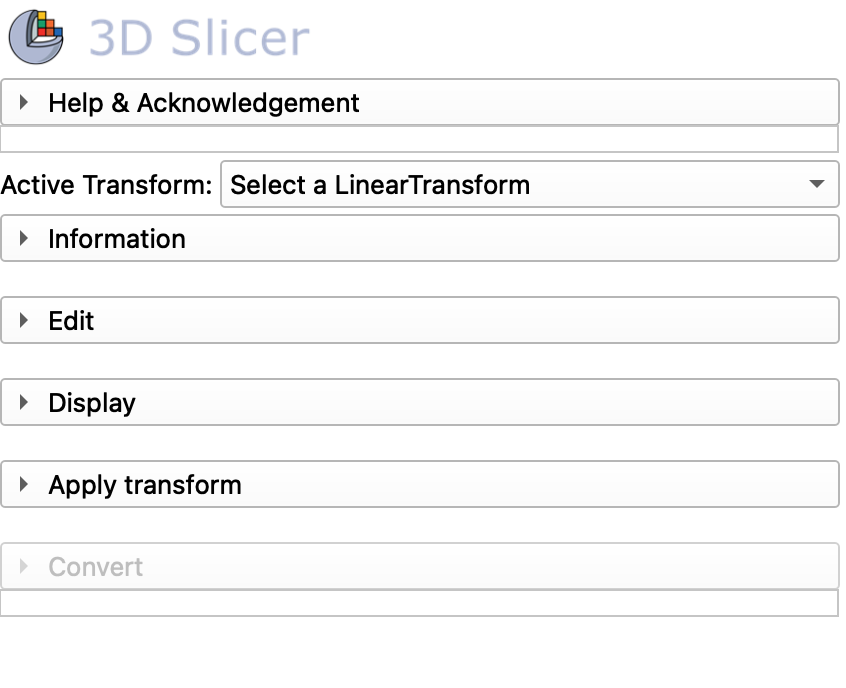
\includegraphics[scale=0.50]{img/modul_example.jpg}
	\captionof{figure}{Das Modul Transforms als Beispiel einer etabliertne 3D Slicer Extension UI | Screenshot aus 3D Slicer}
	\label{fig:module_example}
\end{minipage}

Für die Extension, welche in der vorliegenden Arbeit erstellt werden soll, wird genau
dieser Ansatz gepflegt und somit eine gute Benutzbarkeit des Moduls gewährleistet.
Die speziellen wünsche der konkreten benutzergruppe sollen jedoch nicht zu kurz
kommen.

Für das erstellen einer ersten funktionierenden Extension, bietet Slicer eine sehr
gute Hilfe. 3D Slicer hat hierfür ein eigenes Modul entickelt, das sich \textit{Extention
Wizard} nennt. Dieses Modul gibt eine gute Einführung in die Entwicklung mit Slicer.
Hiermit lässt sich mittels Leitfaden eine erste Demo Extension erstellen, die sich
bereits gut in 3D Slicer einfügt. Diese Lösung könnte als Abstraktionsschicht betrachtet
werden, da durch dieses Modul im ersten Schritt nahe zu keine Kentnisse über die Kernanwendung
von Slicer nötig sind. Der Extentionwizard ist wie folgt zu finden:

\texttt{Modules -> Developer Tools -> Extension Wizard}

Für die Kapselung einer 


% ---------------------------------------------------------------------------------------

\section{Erarbeiten von Lösungsansätzen}
\label{sec:lösungsansätze} hier geht es um Brainstorming

\textbf{Architekturdesign}

\textbf{UI Design}

\textbf{Pseudo Extension}

\textbf{Kappselung Hoffmann}

\textbf{Single Prozess}

\textbf{Batch Prozess}

\textbf{Analysen}
% ---------------------------------------------------------------------------------------

\section{Auswahl von Lösungsansätzen}